\documentclass[11pt]{article}
\usepackage[margin=1.1in]{geometry}
\usepackage{amsmath,amssymb,amsthm}
\usepackage{graphicx}
\usepackage{booktabs}
\usepackage[hidelinks]{hyperref}

\newtheorem{theorem}{Theorem}
\newtheorem{proposition}{Proposition}
\newtheorem{lemma}{Lemma}
\newtheorem{corollary}{Corollary}
\theoremstyle{remark}
\newtheorem{remark}{Remark}

\newcommand{\R}{\mathbb{R}}
\newcommand{\E}{\mathbb{E}}
\newcommand{\Prob}{\mathbb{P}}
\newcommand{\lbar}{\bar{\lambda}}

\title{Softmax from Fast Mixing}
\author{Peter Cotton\thanks{Code and machine verification for every claim in this
paper: \url{https://github.com/microprediction/kinetics} (experiments 7 and 9).
Web companion: \url{https://kinetics.microprediction.org}.}}
\date{August 2026 --- working draft}

\begin{document}
\maketitle

\begin{abstract}
Softmax is used as a choice law almost everywhere, usually without a mechanism
that produces it. We give one. When $N$ channels compete under a shared hidden
state that mixes faster than the channels fire, the winning probability is
softmax in the stationary mean intensities at leading order, and the first
correction is a Green--Kubo term built from integrated rate autocovariances.
One pair of objects, the mean intensities and the correlation matrix $K$, then
predicts every blocked-subset counterfactual by restricting sums, so the whole
deletion ensemble follows from one calculation. Fluctuations common to all
channels cancel exactly, so departures from softmax measure differential
structure alone, and environmental modes of rank $r$ give $K$ of rank exactly
$r$. We verify the expansion on finite chains, then on Brownian narrow escape
with reaction windows, where the leading and corrected errors decay with
measured orders $0.93$ and $1.93$ against an exactly discretized generator.
\end{abstract}

\section{Introduction}

A choice among competing options is often modelled by softmax. The rule assigns
option $i$ a probability proportional to $e^{\theta_i}$, and it appears in
discrete choice, reinforcement learning, statistical physics, and the output
layer of essentially every classifier. Its usual justification is
convenience. Softmax is smooth, normalized, and differentiable, and in the
Gumbel random-utility model it is exact.

Underneath many applications, though, there is real kinetics. A chemical
reaction fires when one of several channels crosses a barrier first. A
diffusing particle escapes through whichever window it encounters first. A
kinetic Monte Carlo (KMC) step selects among escape channels by their rates.
In these systems the choice is a race, and the race has a mechanism. It is
worth asking what that mechanism implies about the choice law, rather than
assuming softmax and moving on.

This paper answers that for one specific and common situation. The channels
share a hidden state, and that state mixes fast relative to the rate at which
channels fire. Catalysis supplies the picture. Adsorbate configurations
rearrange quickly while the reaction event is rare, so every channel sees an
environment that has effectively averaged out. Under that separation we show
two things.

The leading-order result is that softmax is exact in the limit, with
$\theta_i = \log \lbar_i$ the log of the stationary mean intensity. Fast
mixing homogenizes the environment, each channel is left with its average
rate, and the race among constant rates is the exponential race, whose choice
law is Luce.

The first correction is a Green--Kubo term. It is built from
$K_{jk} = \int_0^\infty \mathrm{Cov}_\pi(\lambda_j(Y_0), \lambda_k(Y_t))\,dt$,
the time-integrated covariance of the firing intensities under the stationary
law. This is a dynamical object rather than a static one. Two channels whose
rates are correlated at equal times contribute nothing unless the correlation
persists over the timescale on which the environment decorrelates.

The correction is what breaks independence of irrelevant alternatives (IIA).
Softmax redistributes a removed channel's probability in proportion to the
survivors' probabilities, which is the IIA prediction and is usually wrong in
physical systems. The Green--Kubo term supplies the deviation, and it does so
for every blocked subset at once.

That last point is the practical one. The pair $(\lbar, K)$ is computed once.
Any counterfactual, remove channel $3$, block channels $\{2,5,7\}$, is answered
by restricting the sums in the correction to the surviving set. No new solve
is required per counterfactual. This is the statistical counterpart of a
theme running through our related work, that one global computation can contain
an entire leave-one-out ensemble.

Two structural facts sharpen the result. Fluctuations shared by all channels,
$\lambda_i(y) = a_i c(y)$, cancel from the correction identically. We show this
is not merely an asymptotic statement. A common fluctuation is a common time
change, so Luce holds exactly at every degree of separation, which is the
proportional-hazards normal form. Separately, if the intensity deviations are
driven by $r$ environmental modes then $K$ has rank exactly $r$, so the
correction inherits any low-dimensional structure the physics has.

Section~\ref{sec:model} sets up the shared-state race and the killed resolvent.
Section~\ref{sec:theory} states and proves the expansion.
Section~\ref{sec:properties} collects the three structural properties.
Section~\ref{sec:chain} verifies everything on finite chains, where each
quantity is an exact linear solve. Section~\ref{sec:escape} moves to
continuous physics, a reflected Brownian motion in a disk with reaction
windows, and reports the measured convergence orders together with two
systematic errors that a layered numerical design exposed.

\section{The shared-state race}\label{sec:model}

Let $Y_t$ be an ergodic Markov process on a state space with generator
$L/\varepsilon$ and invariant law $\pi$. The parameter $\varepsilon$ is the
ratio of the environment's mixing time to the timescale on which channels
fire. Small $\varepsilon$ means fast mixing.

Each channel $i \in \{1, \dots, N\}$ fires at intensity $\lambda_i(Y_t) \ge 0$,
conditionally Poisson given the path of $Y$. The first channel to fire wins.
For an available set $A \subseteq \{1, \dots, N\}$ write
$\Lambda_A(y) = \sum_{j \in A}\lambda_j(y)$ for the total hazard, and write
$\lbar_i = \int \lambda_i \, d\pi$ for the stationary mean intensity.

Let $u_i^A(y)$ be the probability that channel $i$ wins, started from $Y_0 = y$.
Conditioning on the first instant and using the conditional Poisson structure
gives
\begin{equation}\label{eq:resolvent}
  \left(\frac{L}{\varepsilon} - \Lambda_A\right) u_i^A = -\lambda_i ,
  \qquad
  u_i^A = \left(\Lambda_A - \frac{L}{\varepsilon}\right)^{-1}\lambda_i .
\end{equation}
This is a killed resolvent. The generator propagates the environment and the
multiplication operator $\Lambda_A$ kills paths at the total firing rate. On a
finite state space it is a linear system, which is what makes the verification
in Section~\ref{sec:chain} exact.

The observable of interest is the win probability from a stationary start,
\begin{equation}\label{eq:p}
  p_i^A = \int u_i^A \, d\pi .
\end{equation}
Summing \eqref{eq:resolvent} over $i \in A$ gives $\sum_{i \in A} u_i^A = 1$,
so the $p_i^A$ are a probability vector on $A$ for every $\varepsilon$.

\section{Homogenization and the Green--Kubo correction}\label{sec:theory}

Write $\tilde\lambda_i = \lambda_i - \lbar_i$ for the fluctuation of the $i$th
intensity, and $\Pi$ for the projection $\Pi f = (\int f d\pi)\mathbf{1}$ onto
constants. The deviation operator
\begin{equation}\label{eq:deviation}
  D = (\Pi - L)^{-1}(I - \Pi)
\end{equation}
inverts $L$ on the mean-zero subspace, and $Dg = \int_0^\infty e^{tL}g \, dt$
for mean-zero $g$. Note the sign it carries. Differentiating that integral
gives $LDg = -g$, so $D$ is minus the pseudo-inverse of $L$, and the sign
propagates into the proof below. The Green--Kubo matrix is
\begin{equation}\label{eq:K}
  K_{jk} = \int_0^\infty \mathrm{Cov}_\pi\!\left(\lambda_j(Y_0),
  \lambda_k(Y_t)\right) dt
  = \int \tilde\lambda_j \, (D\tilde\lambda_k) \, d\pi .
\end{equation}
The second expression is what one computes. It replaces a time integral by a
single linear solve. Note that $K$ need not be symmetric. It is symmetric when
the environment is reversible, and the verification in Section~\ref{sec:chain}
deliberately uses a non-reversible chain so that the index placement in the
theorem is actually tested.

\begin{theorem}[Homogenized choice law and its first correction]\label{thm:main}
Let $\bar\Lambda_A = \sum_{j\in A}\lbar_j$ and suppose $\bar\Lambda_A > 0$.
Then as $\varepsilon \to 0$,
\begin{equation}\label{eq:main}
  p_i^A
  = \frac{\lbar_i}{\bar\Lambda_A}
  - \frac{\varepsilon}{\bar\Lambda_A}
    \left[\sum_{j \in A} K_{ji}
      - \frac{\lbar_i}{\bar\Lambda_A}\sum_{j,k \in A} K_{jk}\right]
  + O(\varepsilon^2) .
\end{equation}
In particular $p_i^A \to \lbar_i / \bar\Lambda_A$, the softmax law in the
log mean intensities $\theta_i = \log\lbar_i$.
\end{theorem}

\begin{proof}
Multiply \eqref{eq:resolvent} by $\varepsilon$ to get
$(L - \varepsilon\Lambda_A)u_i^A = -\varepsilon\lambda_i$, expand
$u_i^A = u^{(0)}_i + \varepsilon u^{(1)}_i + \varepsilon^2 u^{(2)}_i +
O(\varepsilon^3)$, and collect powers of $\varepsilon$.

At order $\varepsilon^0$, $L u^{(0)}_i = 0$, so $u^{(0)}_i$ is a constant
$c_i$ by ergodicity.

At order $\varepsilon^1$ the equation reads
$L u^{(1)}_i = \Lambda_A c_i - \lambda_i$. A solution exists only if the right
side is orthogonal to $\pi$, which forces $\bar\Lambda_A c_i = \lbar_i$ and
gives the leading term. The right side is then
$c_i\tilde\Lambda_A - \tilde\lambda_i$ with
$\tilde\Lambda_A = \sum_{j\in A}\tilde\lambda_j$, and inverting with $LD = -I$
on mean-zero functions gives
\[
  u^{(1)}_i = -D\!\left(c_i \tilde\Lambda_A - \tilde\lambda_i\right) + m_i ,
\]
where the constant $m_i = \int u^{(1)}_i d\pi$ is fixed at the next order.

At order $\varepsilon^2$ the equation is
$L u^{(2)}_i = \Lambda_A u^{(1)}_i$, whose solvability condition is
$\int \Lambda_A u^{(1)}_i \, d\pi = 0$. The constant part of $\Lambda_A$
contributes $\bar\Lambda_A m_i$, the constant $m_i$ integrates against
$\tilde\Lambda_A$ to zero, and what remains is
\[
  0 = \bar\Lambda_A m_i
      - \int \tilde\Lambda_A \, D\!\left(c_i\tilde\Lambda_A
        - \tilde\lambda_i\right) d\pi .
\]
Using \eqref{eq:K}, $\int \tilde\Lambda_A D \tilde\lambda_i \, d\pi
= \sum_{j\in A} K_{ji}$ and
$\int \tilde\Lambda_A D \tilde\Lambda_A \, d\pi = \sum_{j,k\in A} K_{jk}$, so
\[
  m_i = -\frac{1}{\bar\Lambda_A}
        \left[\sum_{j\in A}K_{ji}
        - \frac{\lbar_i}{\bar\Lambda_A}\sum_{j,k\in A}K_{jk}\right].
\]
Finally $p_i^A = c_i + \varepsilon m_i + O(\varepsilon^2)$ by \eqref{eq:p},
which is \eqref{eq:main}.
\end{proof}

\begin{remark}
The two terms in the bracket have distinct roles. The first,
$\sum_{j\in A}K_{ji}$, measures how channel $i$'s rate correlates dynamically
with the total hazard it competes against. The second subtracts the part of
that effect which is common to all channels, and is what keeps
$\sum_{i\in A}p_i^A = 1$ at each order.
\end{remark}

\section{Three structural properties}\label{sec:properties}

\paragraph{One computation answers every counterfactual.} The pair
$(\lbar, K)$ does not depend on $A$. Every blocked-set counterfactual is
obtained from \eqref{eq:main} by restricting the sums to the surviving set.
For a system with $N$ channels this replaces $2^N$ separate resolvent solves
with one deviation solve and $O(N^2)$ stored numbers.

\paragraph{Common-mode fluctuations cancel.} Suppose
$\lambda_i(y) = a_i c(y)$, so that every channel is modulated by the same
environmental factor. Then $\tilde\lambda_i = a_i \tilde{c}$ and
$K_{jk} = a_j a_k \gamma$ with $\gamma = \int \tilde c \, (D\tilde c)\, d\pi$.
Substituting into the bracket in \eqref{eq:main} gives
$a_i \gamma \sum_{j\in A} a_j - (a_i/\sum_{j\in A}a_j)\gamma
(\sum_{j\in A}a_j)^2 = 0$. The correction vanishes identically.

\begin{proposition}[Proportional hazards give Luce exactly]\label{prop:common}
If $\lambda_i(y) = a_i c(y)$ with $c > 0$ then
$p_i^A = a_i / \sum_{j\in A} a_j$ exactly, for every $\varepsilon$ and every
$A$, not merely to the order computed above.
\end{proposition}

\begin{proof}
Let $\tau_c(t) = \int_0^t c(Y_s)\,ds$, a strictly increasing time change. In
the clock $\tau_c$ every channel fires at the constant rate $a_i$, because the
cumulative hazard of channel $i$ up to real time $t$ is $a_i \tau_c(t)$. The
race is then a race among constant exponential rates, whose winner is $i$ with
probability $a_i/\sum_{j\in A}a_j$, independently of the clock. Since the
identity of the winner is invariant under a common monotone time change, the
same holds in real time.
\end{proof}

This is a stronger statement than the vanishing of the correction, and it is
practically useful in the opposite direction. It says a measured departure from
softmax cannot be produced by any amount of shared environmental fluctuation.
Whatever deviation is observed is evidence of differential structure among the
channels.

\paragraph{Low-rank environments give low-rank corrections.} Suppose the
intensity deviations are driven by $r$ environmental modes,
$\lambda_i - \lbar_i = b_i^\top z(y)$ with $z$ taking values in $\R^r$ and
$\int z \, d\pi = 0$. Then $K = B \Gamma B^\top$ with $B$ the $N \times r$
matrix of loadings and $\Gamma_{ab} = \int z_a (D z_b) d\pi$, so $K$ has rank
at most $r$. The compressed correlated race that appears elsewhere in this
program therefore has a physical provenance rather than being a modelling
convenience.

\section{Verification on finite chains}\label{sec:chain}

On a finite state space every object above is an exact linear solve, so the
theorem can be tested without simulation error. Experiment 7 in the repository
runs a six-state chain with ten channels.

The measured convergence order of the leading term is $0.985$, against the
theoretical $1$. After adding the Green--Kubo correction the measured order is
$1.985$, against the theoretical $2$. The gain of exactly one order is the
signature the expansion predicts.

\begin{figure}[t]
  \centering
  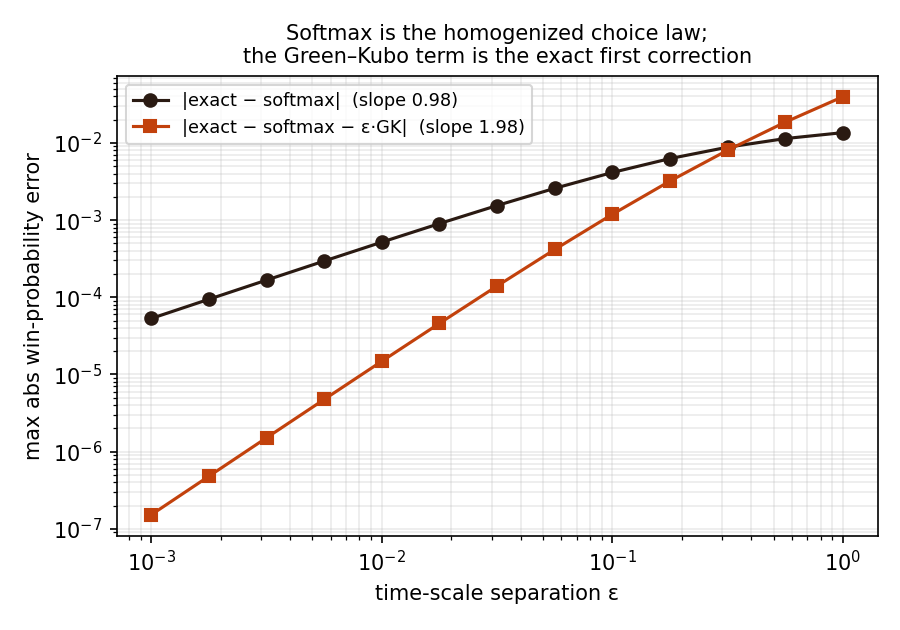
\includegraphics[width=0.49\textwidth]{figs/chain_convergence.png}
  \hfill
  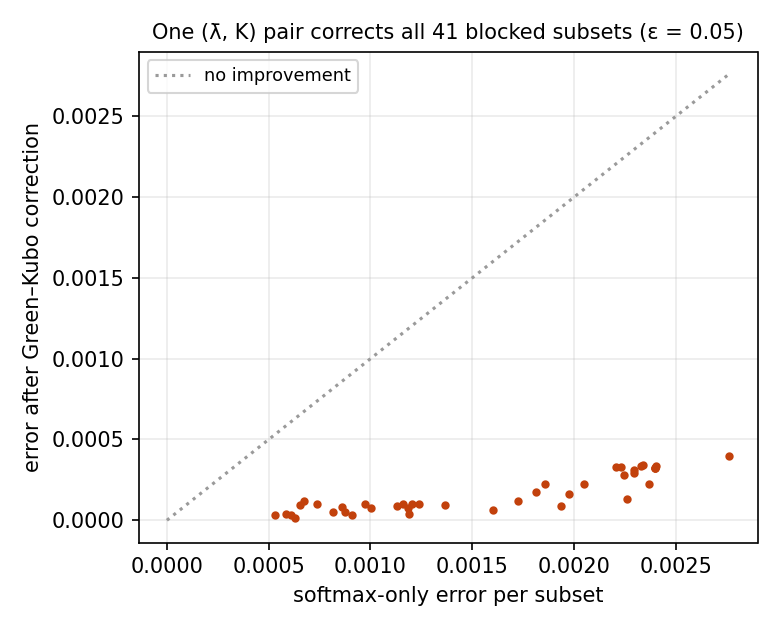
\includegraphics[width=0.49\textwidth]{figs/subsets.png}
  \caption{Finite-chain verification (experiment 7). Left, error against
  $\varepsilon$ for the leading softmax law and for the Green--Kubo corrected
  law, with measured orders $0.985$ and $1.985$. Right, the same $(\lbar, K)$
  pair applied to $41$ random availability sets at $\varepsilon = 0.05$, with
  no per-subset computation.}
  \label{fig:chain}
\end{figure}

The subset-uniformity claim is tested by fixing one $(\lbar, K)$ pair and
predicting $41$ random availability sets at $\varepsilon = 0.05$. The maximum
error over all subsets falls from $2.8\times10^{-3}$ under softmax to
$4.0\times10^{-4}$ with the correction, with no per-subset computation.

Common-mode cancellation is confirmed at $2.6\times10^{-16}$ for the
Green--Kubo coefficient, and the exact win probabilities agree with Luce to
$1.1\times10^{-16}$ at $\varepsilon = 0.3$, which is far outside the asymptotic
regime and is the content of Proposition~\ref{prop:common}. Rank-two
environmental loadings give $K$ with singular values
$[0.022, 0.002, 0, 0]$, so the rank is exactly two.

A Gillespie simulation of the same system, event-driven and including the
hidden state, agrees with the resolvent solution to $1.9\times10^{-3}$ across
$40{,}000$ trajectories at $\varepsilon = 0.3$, which is its own sampling
noise.

An independent reimplementation, written from the statement of
Theorem~\ref{thm:main} alone and run on a deliberately non-reversible chain
where $K$ is asymmetric by $4.0\times10^{-3}$, reproduces the order gain
($0.934$ to $1.935$), matches $K$ against brute-force time integration of the
covariance to $7.7\times10^{-10}$, and reproduces both structural properties.
The non-reversible test matters because it is what distinguishes $K_{ji}$ from
$K_{ij}$ in \eqref{eq:main}.

\section{Narrow escape}\label{sec:escape}

Finite chains verify the algebra. To test the theorem as a statement about
physics we take the hidden state to be reflected Brownian motion in the unit
disk and the channels to be reaction windows on the boundary, bands in which
channel $i$ fires at rate $\kappa$. The first window to fire wins. Here
$\kappa$ plays the role of $\varepsilon$, since a slow reaction rate means the
particle mixes many times before firing.

Experiment 9 separates three layers so that no error source can hide in
another. Layer A is a real Brownian simulation with independent per-step
firing. Layer B is an exact killed-resolvent solve on a finite-volume Neumann
Laplacian over a polar grid, with the uniform invariant law, reversibility, and
conservation asserted numerically rather than assumed. Layer C is the theory,
band-area softmax plus the Green--Kubo term from one deviation solve, using the
same code that passed the chain tests.

Comparing layers B and C tests the theorem on a continuous-physics generator.
The softmax error decays with measured order $0.93$ and the corrected error
with order $1.93$, again a clean gain of one order. At $\kappa = 2$ the
correction takes the maximum error from $1.6\times10^{-3}$ to
$5.0\times10^{-5}$.

\begin{figure}[t]
  \centering
  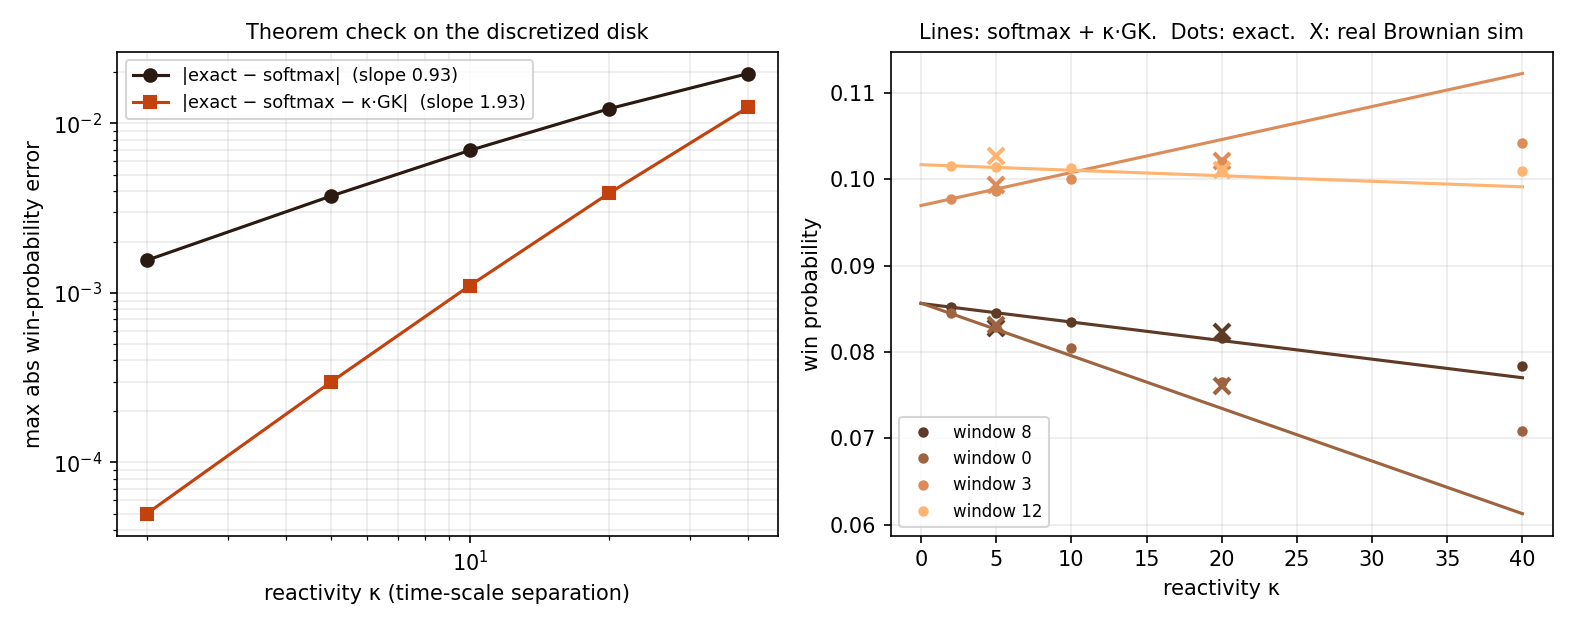
\includegraphics[width=0.62\textwidth]{figs/gk_continuous.png}
  \caption{The theorem on continuous physics (experiment 9). Reflected
  Brownian motion in the unit disk with boundary reaction windows, error
  against $\kappa$ for the leading and corrected laws, measured orders $0.93$
  and $1.93$ against an exactly discretized Neumann generator.}
  \label{fig:continuous}
\end{figure}

Comparing layers A and B tests the discretization. The maximum discrepancy is
$2.2\times10^{-3}$ at $\kappa = 5$ with $50{,}000$ trajectories against a
sampling noise of about $10^{-3}$, and falls to $9.6\times10^{-4}$ against a
noise floor of $7\times10^{-4}$ in a $200{,}000$-trajectory check.

\paragraph{Two systematic errors the layering caught.} Both would have
corrupted a direct comparison of simulation against theory, and neither is
visible without the middle layer.

The first is band quantization, worth $5\times10^{-2}$. Sharp cell indicators
mis-size any window narrower than a grid cell, by up to a factor of three.
Fractional area-exact cell coverage fixes it, after which band areas match
their analytic values to $10^{-14}$.

The second is overlap semantics, worth $1.4\times10^{-2}$. The window geometry
contains three overlapping pairs. The original simulation awarded an overlap to
the lower-indexed window, while the model stacks intensities as
$\lambda = \kappa \sum_i g_i$, which is the physically correct convention for
independent receptors. The error's structure identified it, being $-0.014$ on
one window and $+0.006$ on its overlap partner, and its flatness under both
time-step and grid refinement confirmed that it was not a discretization
artifact.

\section{Discussion}

The result explains why softmax is a reasonable default in systems with fast
shared dynamics, and it quantifies exactly when that default fails. The failure
is governed by integrated dynamical correlations, not by static ones, and it is
insensitive to any fluctuation shared across channels.

Three limitations bound the claim. The expansion is in the mixing-to-firing
timescale ratio and says nothing when channels fire faster than the environment
relaxes. The correction is first order, so systems at moderate separation
retain an $O(\varepsilon^2)$ residual, visible in the finite-$\kappa$ end of
Section~\ref{sec:escape}. The results are proved for finite chains and verified
on a reversible diffusion, and a formal treatment of reversible diffusions with
a spectral gap is left open.

Two extensions look tractable. The disk's boundary operator diagonalizes in
Fourier modes, which may render the leading geometric correction analytic
rather than numerical. Separately, the Green--Kubo kernel and the empirical
substitution kernel of the companion work describe the same non-IIA structure
from theory and from data, and identifying them would connect a computed
correction to an estimated one.

\end{document}
